\documentclass[letterpaper,10pt]{article}

\usepackage{titling}
\usepackage{listings}
\usepackage{url}
\usepackage{setspace}
\usepackage{subfig}
\usepackage{sectsty}
\usepackage{pdfpages}
\usepackage{colortbl}
\usepackage{multirow}
\usepackage{multicol}
\usepackage{relsize}
\usepackage{amsmath}
\usepackage{fancyvrb}
\usepackage[yyyymmdd]{datetime}
\usepackage{amsmath,amssymb,amsthm,graphicx,xspace}
\usepackage[titlenotnumbered,noend,noline]{algorithm2e}
\usepackage[compact]{titlesec}
\usepackage{XCharter}
\usepackage[T1]{fontenc}
\usepackage{tikz}
\usetikzlibrary{arrows,automata,shapes,trees,matrix,chains,scopes,positioning,calc}
\tikzstyle{block} = [rectangle, draw, fill=blue!20, 
    text width=2.5em, text centered, rounded corners, minimum height=2em]
\tikzstyle{bw} = [rectangle, draw, fill=blue!20, 
    text width=4em, text centered, rounded corners, minimum height=2em]

\definecolor{namerow}{cmyk}{.40,.40,.40,.40}
\definecolor{namecol}{cmyk}{.40,.40,.40,.40}
\renewcommand{\dateseparator}{-}


\let\LaTeXtitle\title
\renewcommand{\title}[1]{\LaTeXtitle{\textsf{#1}}}


\newcommand{\handout}[5]{
  \noindent
  \begin{center}
  \framebox{
    \vbox{
      \hbox to 5.78in { {\bf ECE252: Systems Programming and Concurrency } \hfill #2 }
      \vspace{4mm}
      \hbox to 5.78in { {\Large \hfill #4  \hfill} }
      \vspace{2mm}
      \hbox to 5.78in { {\em #3 \hfill \today } }
    }
  }
  \end{center}
  \vspace*{4mm}
}

\newcommand{\lecture}[3]{\handout{#1}{#2}{#3}{Lecture #1}}{
\newcommand{\tuple}[1]{\ensuremath{\left\langle #1 \right\rangle}\xspace}

\addtolength{\oddsidemargin}{-1.000in}
\addtolength{\evensidemargin}{-0.500in}
\addtolength{\textwidth}{2.0in}
\addtolength{\topmargin}{-1.000in}
\addtolength{\textheight}{1.75in}
\addtolength{\parskip}{\baselineskip}
\setlength{\parindent}{0in}
\renewcommand{\baselinestretch}{1.5}
\newcommand{\term}{Spring 2019}

\singlespace


\begin{document}

\lecture{ 14 --- Synchronization Patterns}{\term}{Jeff Zarnett}

\section*{Synchronization Patterns}

There are a number of common synchronization patterns that occur frequently and we can use semaphores to solve them. These synchronization patterns are ways of co-ordinating two threads or processes. We have already examined serialization and mutual exclusion, but there are many more. Throughout this section we will use pseudocode and something like ``Statement A1'' could be any valid statement in the program; what exactly it does is not important as the semaphore is a general solution. The examples in this section come from~\cite{lbs}.

\subsection*{Signalling}
Recall from earlier the example with Alice and Bob at the power plant. This was signalling: Bob sends a signal to Alice to indicate that he has arrived to work and Alice may go home. Signalling can be used in general as a way of indicating that something has happened. Suppose we have a semaphore named \texttt{sem}, initialized to 0.

\begin{multicols}{2}
\textbf{Thread A}\vspace{-2em}
  \begin{verbatim}
	1. Statement A1
	2. signal( sem )
  \end{verbatim}
\columnbreak
\textbf{Thread B}\vspace{-2em}
  \begin{verbatim}
	1. wait( sem )
	2. Statement B2
  \end{verbatim}
\end{multicols}
\vspace{-2em}

If $B$ gets to the \texttt{wait} statement first, it will be blocked (as the semaphore is 0) and cannot proceed until someone signals on that semaphore. When $A$ does call \texttt{signal}, then $B$ may proceed. If instead $A$ gets to the \texttt{signal} statement first, it will signal and the semaphore value will be 1. Then, when $B$ gets to the \texttt{wait} statement, it can proceed without delay. Regardless of the actual order that the threads run, we are certain that statement A1 will execute before statement B2.

Note that this is a situation where it makes sense for a thread to signal a semaphore even if it is not the thread that waited on that semaphore. Thus, sometimes, the semaphore is appropriate and the mutex structure is not necessary in every circumstance.

\subsection*{Rendezvous}
The rendezvous is an expansion of the signal pattern so that it works both ways: two threads should be at the same point before either of them may proceed (they ``meet up''). Given the following code:

\begin{multicols}{2}
\textbf{Thread A}\vspace{-2em}
  \begin{verbatim}
	1. Statement A1
	2. Statement A2
  \end{verbatim}
\columnbreak
\textbf{Thread B}\vspace{-2em}
  \begin{verbatim}
	1. Statement B1
	2. Statement B2
  \end{verbatim}
\end{multicols}
\vspace{-2em}

The desirable property is that A1 should take place before B2 and that B1 should take place before A2. As each thread must wait for the other, two semaphores will be needed: one to indicate that $A$ has arrived and one for $B$. We will assign them the names \texttt{aArrived} and \texttt{bArrived} and initialize both to 0. A first attempt at a solution:

\begin{multicols}{2}
\textbf{Thread A}\vspace{-2em}
  \begin{verbatim}
	1. Statement A1
	2. wait( bArrived )
	3. signal( aArrived )
	4. Statement A2
  \end{verbatim}
\columnbreak
\textbf{Thread B}\vspace{-2em}
  \begin{verbatim}
	1. Statement B1
	2. wait( aArrived )
	3. signal( bArrived )
	4. Statement B2
  \end{verbatim}
\end{multicols}
\vspace{-2em}


The problem here should be obvious: thread $A$ gets to the \texttt{wait} statement and will wait until $B$ signals its arrival before it can proceed. Thread $B$ gets to its \texttt{wait} statement and will wait until $A$ signals its arrival before it will proceed. Unfortunately, each thread is waiting for the other to signal and neither of them can get to the actual \texttt{signal} statement because they are both blocked. 

Neither thread can proceed. The situation can never be resolved, because there is no external force (e.g., a hardware interrupt that means the data has been read from a device) that would cause one or the other to be unblocked. This is a situation called \textit{deadlock}, and it is a subject that will receive a great deal of examination later on. For now, an informal definition is: all threads are permanently stuck. Obviously, this is undesirable.

What if instead, the threads reverse the order and signal first before waiting?

\begin{multicols}{2}
\textbf{Thread A}\vspace{-2em}
  \begin{verbatim}
	1. Statement A1
	2. signal( aArrived )
	3. wait( bArrived )
	4. Statement A2
  \end{verbatim}
\columnbreak
\textbf{Thread B}\vspace{-2em}
  \begin{verbatim}
	1. Statement B1
	2. signal( bArrived )
	3. wait( aArrived )
	4. Statement B2
  \end{verbatim}
\end{multicols}
\vspace{-2em}

This solution works: if $A$ gets to the rendezvous point first, it signals its arrival and waits for $B$. If $B$ gets there first, it signals its arrival and waits for $A$. Whichever gets there last will signal and unblock the other, before it calls \texttt{wait} and will be able to proceed directly because the first thread to arrive already signalled. 

A variation on this can also work where only one thread signals first and the other thread signals second. This is shown below:

\begin{multicols}{2}
\textbf{Thread A}\vspace{-2em}
  \begin{verbatim}
	1. Statement A1
	2. wait( bArrived )
	3. signal( aArrived )
	4. Statement A2
  \end{verbatim}
\columnbreak
\textbf{Thread B}\vspace{-2em}
  \begin{verbatim}
	1. Statement B1
	2. signal( bArrived )
	3. wait( aArrived )
	4. Statement B2
  \end{verbatim}
\end{multicols}
\vspace{-2em}

While this solution will not result in deadlock, it is somewhat less efficient than the previous: it may require an extra switch between processes. If $A$ arrives at the \texttt{wait} statement, it waits; then $B$ signals and must then wait for $A$'s signal (it cannot proceed right away even though it got there second). After $A$ gets to run again it may proceed to signal and unblock $B$. For the most part, we are usually satisfied as long as we are certain that deadlock will not occur that a given solution is acceptable. Nevertheless, the previous solution is provably better and is what programmers want to implement.

\subsection*{Mutual Exclusion}
We saw previously the motivation and concept of mutual exclusion through messages in the linked list example. The general form in pseudocode is of course:

\begin{multicols}{2}
\textbf{Thread A}\vspace{-2em}
  \begin{verbatim}
	1. wait( mutex )
	2. critical section
	3. signal( mutex )
  \end{verbatim}
\columnbreak
\textbf{Thread B}\vspace{-2em}
  \begin{verbatim}
	1. wait( mutex )
	2. critical section
	3. signal( mutex )
  \end{verbatim}
\end{multicols}
\vspace{-2em}

The mutex semaphore is originally initialized to 1 (unlike the previous examples where it started at 0), so whichever thread gets to the \texttt{wait} statement first will proceed immediately and not be blocked at all. If the semaphore were initialized to 0 then neither thread could ever get to the \texttt{signal} statement or ever get into the critical section (deadlock).

Note that both threads $A$ and $B$ are identical here, which was not always the case in previous examples. This is a \textit{symmetric} solution. It is easier to make predictions about the behaviour of the threads when they all do the same thing. If the different threads have different sections of code, they are \textit{asymmetric}. The symmetric solutions very often scale well: we could have arbitrarily many threads executing in that same pattern, as long as they all wait on the semaphore before entering the critical section, we can be sure mutual exclusion is enforced.

\subsection*{Multiplex}
In addition to the binary semaphore, we also discussed the general semaphore. If the general semaphore is initialized to $n$, then at most $n$ threads can be in the critical section at a time. This pattern is more common than it might appear at first glance. Restaurants have a certain number of tables and seats. If more people wish to dine than there are seats available, those customers must wait until some seats become available (other customers leave). Restaurants generally want to pack in as many seats as possible, but fire safety regulations set a maximum occupancy for a given space.

In a computer related example, suppose that the system has a problem that when too many concurrent database requests are happening. The queries become slow and eventually time out. A potential solution is to protect all database accesses with a binary semaphore, so only one database query can run at any time. Analysis may reveal that this is too restrictive a policy; perhaps we can execute 5 queries concurrently without any slowdown. Then initialize the semaphore with a value of 5, allowing at most 5 threads into the critical section at any time.

Now, to represent this in pseudocode. This is a symmetric solution, so it will work for arbitrarily many threads (and showing $A$ and $B$ side by side is not necessary).

\textbf{Thread \textit{K}}\vspace{-2em}
  \begin{verbatim}
	1. wait( mutex )
	2. critical section
	3. signal( mutex )
  \end{verbatim}
\vspace{-2em}

This looks exactly like the solution for mutual exclusion, as it should. The only difference is how many threads can enter the critical section at a time (1 vs. many). 


\subsection*{Barrier}
The barrier pattern is a generalization of the rendezvous pattern; a way of having more than two threads meet up at the same point before any can proceed. Given $n$ threads, each of which knows that the total number of threads is $n$, when the first $n-1$ threads arrive, they should wait until the $n$th arrives. As a solution we might consider a variable to keep track of the number of threads that have reached the appropriate point. Because this variable is shared data, modification of it should be in a critical section.  Thus we will have a semaphore, initialized to 1, called \texttt{mutex} to protect that counter. Then we will have a second semaphore, \texttt{barrier} that will be the place where threads wait until the $n$th thread arrives.


\textbf{Thread \textit{K}}\vspace{-2em}
  \begin{verbatim}
	1. wait( mutex )
	2. count++
	3. signal( mutex )
	4. if count == n
	5.     signal( barrier )
	6. end if
	7. wait( barrier )
  \end{verbatim}
\vspace{-2em}

When the $n$th thread arrives, it unlocks the barrier (signals it) and then may proceed. Unfortunately, this is not a solution, because it will lead to some threads being permanently stuck. If there is more than one thread waiting at the barrier, the first thread will be unblocked when the $n$th thread signals on it. However, after that, there are no other \texttt{signal} statements and therefore the other threads waiting are stuck forever, waiting for a signal that will never come.

Perhaps the idea occurred to you that the $n$th thread to arrive should signal $n-1$ times:

\textbf{Thread \textit{K}}\vspace{-2em}
  \begin{verbatim}
	1. wait( mutex )
	2. count++
	3. signal( mutex )
	4. if count == n
	5.     for i from 1 to  n
	6.         signal( barrier )
	7.     end for
	8. end if
	9. wait( barrier )
  \end{verbatim}
\vspace{-2em} 

This is a solution that allows all of the $n$ threads to proceed (none get stuck), but it is less than ideal. The thread that runs last is very likely the lowest priority thread (if it were high priority it would likely have run first) and therefore when it signals on the semaphore, the thread that has just been unblocked will be the next to run. Then the system switches back, at some later time, to the thread currently unblocking all the others. Thus, in the worst case, there are $2n$ process switches, when it could be accomplished with just $n$~\cite{mte241}. Have each thread unblock the next:

\textbf{Thread \textit{K}}\vspace{-2em}
  \begin{verbatim}
	1. wait( mutex )
	2. count++
	3. signal( mutex )
	4. if count == n
	5.     signal( barrier )
	6. end if
	7. wait( barrier )
	8. signal( barrier )
  \end{verbatim}
\vspace{-2em}

This pattern of a wait followed immediately by a signal is a common pattern called a \textit{turnstile}. The analogy should be familiar to anyone who has travelled by subway (e.g., in Toronto or NYC): a turnstile allows one person at a time to go through. A turnstile pattern allows one thread at a time to proceed through, but can be locked to bar all threads from proceeding. Initially the turnstile in the above example is locked, and the $n$th thread unlocks it and permits all $n$ threads to go through.

Alert readers may have noticed something that causes some minor distress: on line 4 in this solution (and the previous, suboptimal one), we are reading the value of \texttt{count}, a shared variable, without the protection of a semaphore. Is this dangerous? Yes, but the alternative is, in this specific instance, worse. Consider this instead:

\textbf{Thread \textit{K}}\vspace{-2em}
  \begin{verbatim}
	1. wait( mutex )
	2. count++
	3. if count == n
	4.     signal( barrier )
	5. end if
	6. wait( barrier )
	7. signal( barrier )
	8. signal( mutex )
  \end{verbatim}
\vspace{-2em}

The problem here is deadlock once again. The first thread waits on \texttt{mutex} and then goes to wait on the \texttt{barrier} semaphore. At this point, the first thread is blocked. When a second thread comes along, it will wait on \texttt{mutex} but can get no further because the first thread has not signalled on it. The counter will be 1, but cannot get past 1. The condition of \texttt{count} equalling $n$ can never be true. Thus, all the threads are stuck. This is a common source of deadlock: blocking on a semaphore while inside a critical region.

\subsection*{The Reusable Barrier}
The barrier solution we have is good (as long as we can live with the read of the \texttt{count} variable outside of a mutual exclusion protection), but the way it is implemented now, \texttt{count} can increase but never decrease. Once the barrier is open, it can never be closed again. Programs very often do the same thing repeatedly, so a one-time use barrier is not ideal; it would be better to have a reusable barrier. One way to deal with this is to decrement \texttt{count} after the rendezvous has taken place. The line labelled ``critical point'' is the section of code that must wait until all the threads have rendezvoused\footnote{In the immortal words of Bill Watterson, author of \textit{Calvin and Hobbes}: ``verbing weirds language.''}.


\textbf{Thread \textit{K}}\vspace{-2em}
  \begin{verbatim}
	 1. wait( mutex )
	 2. count++
	 3. signal( mutex )
	 4. if count == n
	 5.     signal( turnstile )
	 6. end if
	 7. wait( turnstile )
	 8. signal( turnstile )
	 9. [critical point]
	10. wait( mutex )
	11. count--
	12. signal( mutex )
	13. if count == 0
	14.     wait( turnstile )
	15. end if
  \end{verbatim}
\vspace{-2em}

There are two problems with the above implementation. Suppose thread $n-1$ is about to execute line 4 (the comparison of \texttt{count}) and then there is a process switch and the $n$th thread comes to this point. Both of them will find that \texttt{count} is equal to $n$ and therefore both threads will signal the turnstile. The same problem occurs on line 13: more than one thread may wait on the turnstile, resulting in deadlock. Let us fix that:


\textbf{Thread \textit{K}}\vspace{-2em}
  \begin{verbatim}
	 1. wait( mutex )
	 2. count++
	 3. if count == n
	 4.     signal( turnstile )
	 5. end if
	 6. signal( mutex )
	 7. wait( turnstile )
	 8. signal( turnstile )
	 9. [critical point]
	10. wait( mutex )
	11. count--
	12. if count == 0
	13.     wait( turnstile )
	14. end if
	15. signal( mutex )
  \end{verbatim}
\vspace{-2em}

This solves the problem previously identified by putting the checks of \texttt{count} inside the critical section controlled by \texttt{mutex}. Unfortunately, there is another problem that can occur here: suppose one particular thread gets through the second mutex but is running in a loop and gets back through the first mutex again. This would be like one thread being one ``lap'' ahead of the others. We can prevent this by having two turnstiles: first all threads wait at the first turnstile until the last gets there and lets them through. Then all threads wait at a second turnstile until the last gets there and lets them all through again. The form of the solution represented visually, is:

\begin{center}
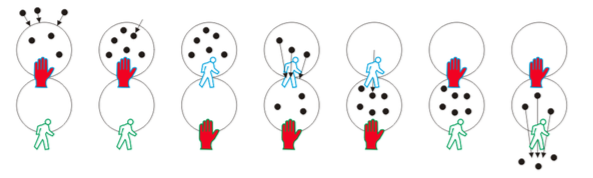
\includegraphics[width=0.75\textwidth]{images/reusable-barrier.png}\\
	A visual representation of the group rendezvous with two turnstiles~\cite{mte241}.
\end{center}

From left to right, the seven steps of the diagram are~\cite{mte241}:
\begin{enumerate}
	\item The threads arrive at the rendezvous.
	\item The $n$th thread arrives at the rendezvous.
	\item That last thread unlocks the first turnstile and locks the second turnstile.
	\item The threads pass through the first turnstile.
	\item The $n$th thread passes through the first turnstile; it may not have been the last to arrive at the first turnstile.
	\item The thread that just arrived locks the first turnstile and unlocks the second.
	\item The threads leave the rendezvous.
\end{enumerate}

\textbf{Thread \textit{K}}\vspace{-2em}
  \begin{verbatim}
	 1. wait( mutex )
	 2. count++
	 3. if count == n
	 4.     wait( turnstile2 )
	 5.     signal( turnstile1 )
	 6. end if
	 7. signal( mutex )
	 8. wait( turnstile1 )
	 9. signal( turnstile1 )
	10. [critical point]
	11. wait( mutex )
	12. count--
	13. if count == 0
	14.     wait( turnstile1 )
	15.     signal( turnstile2 )
	16. end if
	17. signal( mutex )
	18. wait( turnstile2 )
	19. signal( turnstile2 )
  \end{verbatim}
\vspace{-2em}

This solution can also be called a \textit{two-phase barrier} because all threads have to wait twice: once at each turnstile.

%\subsection*{Queue}
%The final synchronization pattern we will examine is the queue. Imagine the road test procedure for getting a driver's license. This requires a trip to the ministry of transportation to meet up with an examiner; then a driver will drive the vehicle around with the examiner in the passenger seat, and the examiner evaluates the driver's performance. At the test centre, there are two queues: one for drivers and one for examiners. When a driver arrives and wants to take the test, if there is an examiner available, they may proceed; otherwise the driver has to wait. If it is an unusually slow day and the examiner gets to the front of the queue and there are no drivers ready to take the test, the examiner has to wait. We will need two semaphores to implement this.

\bibliographystyle{alphaurl}
\bibliography{252}


\end{document}
